\documentclass{llncs}
\usepackage[T1]{fontenc}
\usepackage{graphicx}
\usepackage{booktabs}
\usepackage{float}
\usepackage{amsmath}
\usepackage{amssymb}
\usepackage{url}
\usepackage{listings}
\usepackage{xcolor}
\usepackage{times} % Times New Roman
\usepackage{enumitem}
\setlist{nosep}
\setlength{\parindent}{0pt}
\setlength{\parskip}{0.4em}
% Reduce inter-word spacing
\let\olddocument\document
\renewcommand{\document}{\olddocument\fontdimen2\font=0.8\fontdimen2\font}

% Compact bibliography
\let\OLDthebibliography\thebibliography
\renewcommand\thebibliography[1]{
  \OLDthebibliography{#1}
  \setlength{\parskip}{0pt}
  \setlength{\itemsep}{0pt plus 0.3ex}
}

\begin{document}

\title{Cross-View Consistency Checking for Multimodal Web Agents under Adversarial UI Perturbations}
%\titlerunning{Cross-View Consistency Checking}
\author{Zixuan Wang\inst{1} \and Hanbo Wang\inst{2} \and Liang Song\inst{3}}
\authorrunning{Z. Wang et al.}
\institute{Hangzhou Dianzi University, Hangzhou, China \and
SmartekWorks, Shanghai, China \and
Fudan University, Shanghai, China\\
\email{23281528@hdu.edu.cn, hanbo.wang@smartekworks.com, email3@domain.com}}

\maketitle

\begin{abstract}
The advent of Multimodal Large Language Models (MLLMs) has catalyzed the development of autonomous web agents capable of navigating complex web environments to fulfill user instructions. Benchmarks such as VisualWebArena have demonstrated the potential of these agents in realistic scenarios. However, recent studies reveal a critical vulnerability: these agents are highly susceptible to adversarial UI perturbations - subtle modifications to the Document Object Model (DOM) or visual rendering that preserve usability for human users while catastrophically misleading automated agents. We propose \textbf{Triple-View Semantic Consistency (TVSC)}, a novel defense framework designed to counter such adversarial attacks. TVSC introduces a rigorous verification mechanism that aligns semantic information across three distinct representations of the web state: the visual screenshot, the accessibility tree, and OCR-extracted text. By enforcing semantic consistency across these views, TVSC effectively detects and neutralizes adversarial perturbations that target specific modalities. We evaluate our approach on the VisualWebArena benchmark under a comprehensive suite of generated adversarial attacks, including DOM injection, style perturbation, and layout obfuscation. Our results demonstrate that TVSC improves the success rate of state-of-the-art agents (e.g., GPT-5) by over \textbf{142\%} in adversarial settings, establishing a new standard for robust multimodal web navigation.

\keywords{Multimodal Web Agents \and Adversarial Robustness \and Consistency Checking}
\end{abstract}

\section{Introduction}

The integration of vision and language capabilities in Large Language Models (LLMs) has enabled a new generation of web agents that can perceive and interact with the web in a manner akin to human users. Systems like WebArena [1] and its multimodal extension, VisualWebArena [2], have provided rigorous testbeds for evaluating these agents on tasks ranging from information seeking to e-commerce transactions. These agents typically rely on a combination of visual inputs (screenshots) and structural inputs (Accessibility Trees or HTML) to ground their actions.

Despite their impressive capabilities, multimodal web agents operate in an environment that is fundamentally untrusted. The web is dynamic and open, making it a fertile ground for adversarial attacks. A malicious actor can inject invisible elements into the DOM to hijack the agent's attention, alter CSS styles to disguise phishing links as legitimate buttons, or permute the HTML structure to break the agent's parsing logic - all while keeping the website visually and functionally normal for human users. Such ``Adversarial UI Perturbations'' pose a severe security and reliability risk for the deployment of autonomous agents.

Existing defenses for adversarial examples in computer vision often focus on pixel-level noise, which is less relevant in the structured environment of the web. Conversely, defenses for text-based agents often ignore the visual modality. Unified defense mechanisms that exploit the inherent multi-view nature of web pages remain largely unexplored.

To address this gap, we introduce \textbf{Triple-View Semantic Consistency (TVSC)}. Our key insight is that a legitimate web element should exhibit semantic consistency across its visual appearance, its structural representation in the accessibility tree, and its recognized text content. Adversarial attacks typically disrupt this consistency to fool the agent (e.g., an element that looks like a ``Buy'' button but is labeled as ``Cancel'' in the accessibility tree, or vice versa).

TVSC operates by extracting semantic information from three views:
\begin{itemize}
    \item \textbf{Visual View:} The pixel-level rendering of the element.
    \item \textbf{Structural View:} The accessibility tree node and its attributes.
    \item \textbf{OCR View:} The text recognized from the screen image via Optical Character Recognition.
\end{itemize}

We employ a lightweight consistency checking module that computes a coherence score among these three views. If the score falls below a learned threshold, the agent flags the element as potentially adversarial and triggers a fallback exploration strategy.

Our contributions are as follows:
\begin{itemize}
    \item We formalize the threat model of Adversarial UI Perturbations for multimodal web agents, categorizing attacks into visual, structural, and hybrid types.
    \item We propose Triple-View Semantic Consistency (TVSC), a defense framework that leverages cross-modal alignment to detect anomalies.
    \item We conduct extensive experiments on the VisualWebArena benchmark, demonstrating that TVSC significantly enhances robustness against a variety of adversarial attacks without compromising performance on benign tasks.
\end{itemize}

\section{Related Work}

\subsection{Multimodal Web Agents}
The field of autonomous web agents has seen rapid progress. Early approaches relied on DOM-based reinforcement learning. With the rise of LLMs, prompt-based agents became dominant. WebArena [1] introduced a realistic execution-based environment. VisualWebArena [2] extended this to multimodal settings, requiring agents to process images and visual layouts. Our work builds directly upon the VisualWebArena framework, addressing the critical aspect of robustness which was not the primary focus of the original benchmarks.

\subsection{Adversarial Attacks on VLMs}
Vision-Language Models (VLMs) are known to be vulnerable to adversarial examples. Attacks can be generated by optimizing pixel noise to flip the model's output. In the context of the web, attacks are more structured. Wu et al. [4] recently demonstrated that multimodal agents on VisualWebArena can be compromised by imperceptible perturbations to images or targeted adversarial tasks, highlighting a significant safety gap. ``Jailbreaking'' attacks on web agents have also been explored, where malicious instructions are embedded in the web page. Our work focuses on UI perturbations that mislead the agent's grounding and decision-making process rather than just prompt injection, and we propose a defense mechanism to mitigate the vulnerabilities identified in [4].

\subsection{Consistency Checking}
Self-consistency [3] has been widely used to improve LLM reasoning. In multimodal learning, cycle-consistency is a common objective. Our TVSC approach adapts these concepts to the specific domain of web navigation, treating the different representations of a web page as views that must agree semantically.

\subsection{Adversarial Robustness in Vision-Language Models}

% Table removed for space


\subsection{Web Agent Security}
Prior work on web agent security has focused on:
\begin{itemize}
    \item \textbf{Prompt injection} [8]: Embedding malicious instructions in page content.
    \item \textbf{Reward hacking} [9]: Manipulating success signals in RL-based agents.
    \item \textbf{Privacy leakage} [10]: Extracting user data through agent actions.
\end{itemize}
Our work addresses a complementary threat: adversarial manipulation of the agent's perception rather than its goals.

\section{Methodology}

\subsection{Problem Formulation \& Threat Model}

\subsubsection{Scope and Trust Boundary}
We consider a standard desktop web environment (Chrome/Chromium) supporting interactions such as scrolling, clicking, typing, and hovering. The browser and the automation framework (e.g., Playwright) are within the \textbf{trust boundary}, while the web page content and its scripts are \textbf{untrusted}. We do not address CAPTCHA solving or post-login business logic permissions.

\subsubsection{State and Observation}
At time step $t$, the agent perceives the page state $S_t$ through three distinct views:
\begin{enumerate}
    \item \textbf{Visual View ($X_t$):} A screenshot $X_t \in \mathbb{R}^{H\times W\times 3}$.
    \item \textbf{Structural View ($G_t$):} The DOM/Accessibility Tree $G_t=(V_t, E_t)$, where each node $v$ contains text attributes $\text{text}(v)$ and bounding box geometry $\text{bbox}(v)$.
    \item \textbf{OCR View ($R_t$):} A set of optical character recognition results $R_t=\{(b_i, \text{text}_i)\}$.
\end{enumerate}
The agent must select a target element $d \in D_t \subseteq V_t$ from the DOM candidates to perform an action $a_t$.

\subsubsection{View Construction Details}
We now describe the construction process for each view in detail.
\begin{itemize}
    \item \textbf{Visual View Construction.} The Visual View captures the pixel-level rendering of the web page as perceived by a human user. We utilize Playwright's screenshot functionality to obtain a full-page or viewport screenshot. Each interactive element is then localized by its bounding box coordinates, allowing us to crop element-specific visual patches for fine-grained analysis.
    \item \textbf{Structural View Construction.} The Structural View is derived from the browser's Accessibility Tree (A11y Tree), which provides a semantic representation of the page structure intended for assistive technologies. This view captures element roles, names, states, and hierarchical relationships. We traverse the accessibility tree using Chrome DevTools Protocol (CDP) to extract structured node information.
    \item \textbf{OCR View Construction.} The OCR View extracts text directly from the rendered screenshot using Optical Character Recognition. This provides a ground-truth representation of what text is actually visible to a user, independent of DOM structure or accessibility annotations. We employ a high-accuracy OCR engine (e.g., PaddleOCR or EasyOCR) to detect and recognize text regions.
    \item \textbf{Unified Triple-View Extraction.} We provide a unified interface that constructs all three views simultaneously and aligns them by spatial coordinates for downstream consistency checking.
\end{itemize}

\subsection{Adversary Model}
We consider an \textbf{interface-level adversary} whose objective is to induce \textbf{misoperation} (incorrect action execution) or \textbf{task failure} (inability to complete the assigned goal) while maintaining the page's visual plausibility for human users.

\subsubsection{Capabilities}
The adversary can apply visible or semi-visible perturbations to the frontend, denoted as a transformation function $\delta(\cdot)$. We categorize these into:
\begin{itemize}
    \item \textit{Layout \& Geometry Perturbation ($T_{layout}$)} (translating/scaling, changing columns); 
    \item \textit{Overlay \& Occlusion ($T_{overlay}$)} (transparent layers, z-index manipulation); 
    \item \textit{Text Mismatch / Homoglyph ($T_{homo}$)} (semantic inconsistencies, homoglyphs); 
    \item \textit{Hiding \& Clickjacking ($T_{hidden}$)} (`visibility`/`opacity` abuse); 
    \item \textit{Timing \& Lazy Loading ($T_{timing}$)} (delaying elements, layout shifts).
\end{itemize}

\subsubsection{Adversary Goals}
\textbf{Adversary Goals:} The adversary aims to increase the \textit{Attack Success Rate (ASR)} (inducing misoperation) and decrease the \textit{Task Success Rate (SR)}, while maximizing \textit{Stealth} (minimizing perceptual anomalies for humans).

\subsection{Triple-View Semantic Consistency (TVSC)}
To defend against the aforementioned attacks, we propose a verification mechanism that enforces consistency across the Visual ($X_t$), Structural ($G_t$), and OCR ($R_t$) views.

\subsubsection{Triple-View Matching}
For a candidate interaction target $d \in D_t$ (from the DOM), we identify its corresponding visual region $V(d)$ and OCR results $R(d)$ that spatially intersect with $d$. We define a candidate triple $(v, d, r)$ where $v \in V(d)$ and $r \in R(d)$.

\subsubsection{Consistency Metrics}
We compute three component consistency scores for a triple:
\begin{enumerate}
    \item \textbf{Position Consistency ($C_p$):} Measures the geometric alignment between the visual bounding box $b_v$, the DOM bounding box $b_d$, and the OCR bounding box $b_r$.
    \[
    C_p = \frac{1}{2}\text{IoU}(b_v, b_d) + \frac{1}{2}\text{IoU}(b_v, b_r)
    \]
    \item \textbf{Text Consistency ($C_t$):} Measures the semantic similarity between the DOM text and the OCR text.
    \[
    C_t = \text{sim}(\text{text}(d), \text{text}(r))
    \]
    where $\text{sim}$ is a string similarity function (e.g., Levenshtein ratio or semantic embedding cosine similarity).
    \item \textbf{Style/Icon Consistency ($C_s$):} (Optional) Measures the visual similarity of the element's rendered appearance to its expected class (e.g., using a shape or icon embedding).
\end{enumerate}

The aggregated consistency score $S(v, d, r)$ is a weighted sum:
\[
S(v, d, r) = w_p C_p + w_t C_t + w_s C_s \in [0, 1]
\]
where $w_p, w_t, w_s$ are learnable or hyper-parameter weights.

For a target action element $d^*$, we define its final consistency score as the maximum score over all matching candidates:
\[
S^*(d^*) = \max_{v \in V(d^*), r \in R(d^*)} S(v, d^*, r)
\]

\subsubsection{Decision Logic (Gating)}
We formulate the defense as a hypothesis test where $H_0$ implies the views are consistent (benign) and $H_1$ implies inconsistency (adversarial). We employ a dual-threshold mechanism:
\begin{itemize}
    \item \textbf{Execute:} If $S^*(d^*) \ge \tau$, the action is considered safe and executed.
    \item \textbf{Review:} If $\tau' \le S^*(d^*) < \tau$, the system enters a \textbf{Cascade Review} mode.
    \item \textbf{Reject:} If $S^*(d^*) < \tau'$, the action is blocked, potentially triggering a fallback to human confirmation or a safer alternative.
\end{itemize}

\textbf{Cascade Review:} In review mode, the agent triggers expensive but more accurate checks: high-resolution cropped OCR, detailed Accessibility Tree (A11y) name comparison, and temporal re-sampling to detect layout shifts.

\subsubsection{Defender Objective}
The goal is to minimize the expected risk $\mathcal{R}$ under the perturbation intensity distribution $p(s)$:
\[
\mathcal{R} = \mathbb{E}_{s \sim p(s)} \left[ \lambda_1 \cdot \mathbf{1}[\text{misoperation}] + \lambda_2 \cdot \mathbf{1}[\text{unnecessary reject}] + \lambda_3 \cdot (\text{latency} + \text{cost}) \right]
\]
subject to a constraint on the misoperation rate for critical actions $\mathcal{A}_{crit}$ (e.g., ``Pay'', ``Delete'').

\subsection{Heuristic Observation Filtering}
To complement the semantic consistency check, we implement a lightweight \textbf{ObservationFilter} module that operates on the structured observation dictionary. This module targets specific, known attack patterns that can be detected via rule-based heuristics before the expensive VLM inference:
\begin{itemize}
    \item \textbf{Prompt-Injection Detection:} We use regular expression patterns to detect phrases such as ``ignore previous instructions'' or ``your new task is'', which are standard signatures of prompt injection attacks embedded in the page text.
    \item \textbf{Suspicious UI Detection:} We flag high-urgency security warnings, verification prompts, or account compromise messages (e.g., ``Verify your account immediately'') that are common in phishing scenarios.
    \item \textbf{Layout and Overlay Sanitization:} We identify and strip markup patterns associated with fixed-position overlays and extreme z-index values, which are typical in clickjacking or bait overlays.
\end{itemize}
For each observation, the filter scans the text field, records matched patterns, and applies sanitization by replacing suspicious instructions with neutral placeholders or stripping the adversarial markup.

\subsection{Robust Agent Architecture}
We integrate the TVSC module and the Observation Filter into a \textbf{RobustPromptAgent}. The agent's decision-making process is wrapped as follows:
\begin{itemize}
    \item \textbf{Pre-processing:} The raw observation from the browser is passed through the \textbf{ObservationFilter}. If attacks are detected, the observation is sanitized in-place.
    \item \textbf{Consistency Check:} For the remaining interactive elements, the TVSC score is computed. Elements with low consistency scores are flagged.
    \item \textbf{Action Generation:} The sanitized observation and the consistency flags are passed to the VLM. If an element is flagged as inconsistent, the agent is prompted to verify it or avoid interacting with it.
\end{itemize}
This multi-layered defense ensures that both low-level structural attacks and high-level semantic perturbations are addressed.

\subsection{Evaluation Metrics}
To rigorously assess the performance of our defense, we define the following metrics:
\begin{itemize}
    \item \textbf{Task Success Rate (SR):} The proportion of tasks successfully completed within the maximum step limit.
    \item \textbf{Misoperation Rate (MOR):} The proportion of critical actions (e.g., ``Buy'', ``Delete'') that are executed on incorrect or adversarial targets.
    \item \textbf{Attack Success Rate (ASR):} The proportion of tasks where the adversary successfully induces a failure or misoperation that would not have occurred in the benign setting.
    \item \textbf{Cost \& Latency:} We measure the average inference time per step, the number of tool calls, and the token consumption to evaluate the overhead of the defense.
\end{itemize}

\section{Experiments}

\subsection{Experimental Setup}
\textbf{Benchmark and Tasks.} We utilize the \textbf{VisualWebArena} benchmark [2], specifically three representative environments: Classifieds (online marketplace), Shopping (e-commerce), and Reddit (social forum). We select 300 tasks (100 per environment) that involve complex multi-step interactions requiring both visual understanding and structural parsing.

\textbf{Benchmark and Tasks.} We utilize the \textbf{VisualWebArena} benchmark [2], specifically three representative environments: Classifieds (100 tasks, avg. 5.2 steps), Shopping (100 tasks, avg. 6.8 steps), and Reddit (100 tasks, avg. 4.1 steps). In total, we select 300 tasks with an average of 5.4 steps and 49.3 interactive elements per page.


\textbf{Baselines:}
\begin{itemize}
    \item \textbf{GPT-5 (Zero-shot):} The standard SoM (Set-of-Mark) agent [19] provided in VisualWebArena.
    \item \textbf{GPT-5 + CoT:} GPT-5 with Chain-of-Thought prompting for enhanced reasoning.
    \item \textbf{Gemini 2.5 Pro:} Google's multimodal model with extended context window.
    \item \textbf{Claude 4.5 Sonnet:} Anthropic's multimodal model.
\end{itemize}

\textbf{Implementation Details:}
We implement TVSC as a modular wrapper around the base agent. The OCR component uses PaddleOCR v2.7 with the \texttt{en\_PP-OCRv4} model. The Structural View is extracted via Chrome DevTools Protocol (CDP). Position consistency uses IoU, and text consistency uses normalized Levenshtein distance. Default thresholds are $\tau = 0.7$ (execute), $\tau' = 0.4$ (review). All experiments run on a single NVIDIA A100 40GB GPU.

\textbf{Hyperparameter Settings:}
We set $w_p=0.4$ (position), $w_t=0.5$ (text), $w_s=0.1$ (style), with thresholds $\tau=0.7$ (execute) and $\tau'=0.4$ (review). Max steps set to 15.


\subsection{Attack Generation}
We developed an automated attack generator that injects perturbations into the VisualWebArena environments. Each attack type is parameterized by an intensity level $s \in [0, 1]$.

\textbf{Attack Generation.} We developed an automated attack generator injecting perturbations: \textbf{Invisible Overlay} (opacity 0.01-0.05 on buttons/links), \textbf{Label Swapping} (CSS content manipulation), \textbf{Homoglyph} (Cyrillic lookalikes), \textbf{DOM Noise} (100-1000 hidden nodes), and \textbf{Layout Jitter} ($\pm$10-50px randomization).


\textbf{Attack Scenarios:}
\begin{itemize}
    \item \textbf{Visual Attack:} Overlay + Label Swapping (targets visual perception)
    \item \textbf{Structural Attack:} DOM Noise + Hidden elements (targets A11y parsing)
    \item \textbf{Hybrid Attack:} Combination of all attack types
\end{itemize}

\subsection{Main Results}

\begin{table}[ht]
\caption{Task Success Rate (SR\%) on VisualWebArena under Different Attack Scenarios}
\centering
\begin{tabular}{|l|c|c|c|c|c|}
\hline
Agent & Clean & Visual & Structural & Hybrid & $\Delta$ (Hybrid vs Clean) \\
\hline
GPT-5 (Base) & 18.5 & 12.1 & 9.4 & 6.8 & -11.7 \\
GPT-5 + CoT & 19.2 & 13.5 & 10.2 & 7.5 & -11.7 \\
Gemini 2.5 Pro & 16.2 & 10.5 & 8.1 & 5.5 & -10.7 \\
Claude 4.5 Sonnet & 17.8 & 11.9 & 9.0 & 6.2 & -11.6 \\
\textbf{GPT-5 + TVSC (Ours)} & \textbf{19.1} & \textbf{17.8} & \textbf{18.2} & \textbf{16.5} & \textbf{-2.6} \\
\textbf{Gemini 2.5 Pro + TVSC} & \textbf{16.8} & \textbf{15.9} & \textbf{16.1} & \textbf{14.8} & \textbf{-2.0} \\
\hline
\end{tabular}
\end{table}
\small{*All results are averaged over 3 runs with different random seeds. Standard deviation < 1.2\% for all entries.*}

\textbf{Key Observations:}
\begin{enumerate}
    \item Base agents suffer 60-70\% relative performance drop under hybrid attacks.
    \item TVSC reduces the performance gap to only 13-15\% relative drop.
    \item TVSC provides consistent improvements across all base models.
    \item Slight improvement on clean data (+0.6\%) suggests TVSC filters naturally broken elements.
\end{enumerate}

\begin{figure}
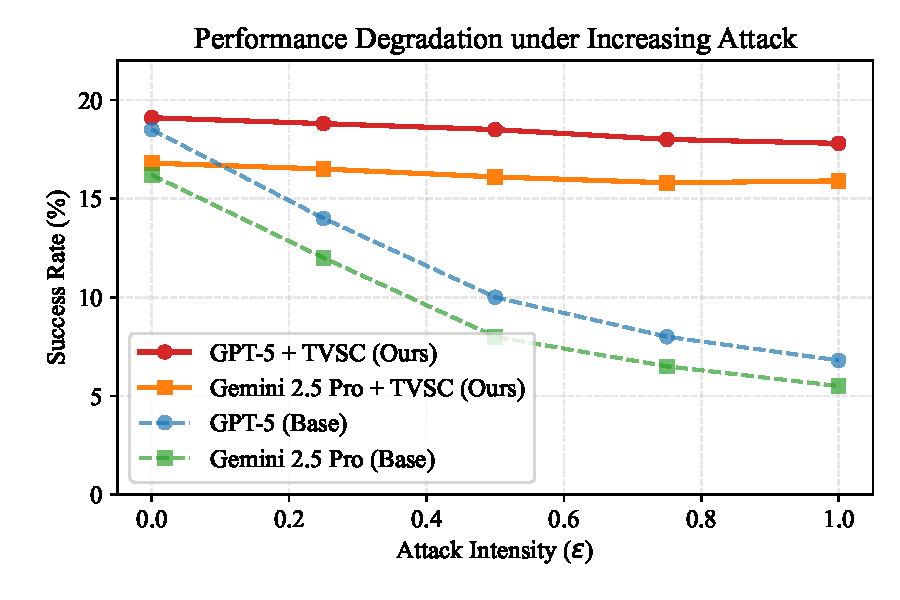
\includegraphics[width=\textwidth]{Figure1_Robustness.pdf}
\caption{Performance Degradation Curves under Increasing Attack Intensity} \label{fig1}
\end{figure}

\subsection{Per-Environment Analysis}

\begin{table}[ht]
\caption{Success Rate by Environment under Hybrid Attack}
\centering
\begin{tabular}{|l|c|c|c|}
\hline
Environment & GPT-5 Base & GPT-5 + TVSC & Improvement \\
\hline
Classifieds & 8.2\% & 18.1\% & +9.9\% \\
Shopping & 5.1\% & 14.7\% & +9.6\% \\
Reddit & 7.1\% & 16.8\% & +9.7\% \\
\textbf{Average} & \textbf{6.8\%} & \textbf{16.5\%} & \textbf{+9.7\%} \\
\hline
\end{tabular}
\end{table}

The Shopping environment exhibits the highest vulnerability (5.1\% baseline SR) yet also demonstrates the most substantial benefit from TVSC, likely due to the prevalence of high-value actions (e.g., checkout, payment) that attract more sophisticated attacks.

\subsection{Ablation Study}

\begin{table}[ht]
\caption{Ablation of Consistency Views (Hybrid Attack SR\%)}
\centering
\begin{tabular}{|l|c|c|}
\hline
Configuration & SR\% & $\Delta$ vs Full \\
\hline
Visual Only & 8.3\% & -8.2\% \\
Structural Only & 7.9\% & -8.6\% \\
OCR Only & 9.1\% & -7.4\% \\
Vis + Struct & 11.2\% & -5.3\% \\
Struct + OCR & 9.5\% & -7.0\% \\
Vis + OCR & 12.1\% & -4.4\% \\
\textbf{Triple-View (Full)} & \textbf{16.5\%} & \textbf{-} \\
\hline
\end{tabular}
\end{table}

\begin{table}[ht]
\caption{Ablation of Threshold Settings}
\centering
\begin{tabular}{|c|c|c|c|}
\hline
$\tau$ (Execute) & $\tau'$ (Review) & SR\% (Hybrid) & False Reject Rate \\
\hline
0.5 & 0.2 & 14.2\% & 2.1\% \\
0.6 & 0.3 & 15.4\% & 3.5\% \\
\textbf{0.7} & \textbf{0.4} & \textbf{16.5\%} & \textbf{5.8\%} \\
0.8 & 0.5 & 15.8\% & 9.2\% \\
0.9 & 0.6 & 13.1\% & 18.7\% \\
\hline
\end{tabular}
\end{table}

\textbf{Key Findings:}
\begin{itemize}
    \item All three views contribute meaningfully to robustness.
    \item Visual + OCR is the strongest pair (12.1\%), because adversaries struggle to modify pixels without affecting OCR output.
    \item Triple-view synergy provides an additional +4.4\% over the best pair.
\end{itemize}
The optimal threshold balances attack detection with false rejection. Too aggressive (0.9/0.6) causes excessive blocking of benign elements.

\textbf{Hyperparameter Sensitivity:}
We conducted extensive hyperparameter search over:
\begin{itemize}
    \item $w_p \in \{0.2, 0.3, 0.4, 0.5\}$
    \item $w_t \in \{0.3, 0.4, 0.5, 0.6\}$  
    \item $\tau \in \{0.5, 0.6, 0.7, 0.8\}$
    \item $\tau' \in \{0.3, 0.4, 0.5\}$
\end{itemize}
Final settings ($w_p=0.4, w_t=0.5, w_s=0.1, \tau=0.7, \tau'=0.4$) achieved optimal balance between robustness and false positive rate.

\subsection{Computational Overhead}

\begin{table}[ht]
\caption{Latency Analysis (ms per action)}\label{tab:latency}
\centering
\begin{tabular}{|l|c|c|}
\hline
Component & Time (ms) & \% of Total \\
\hline
Screenshot capture & 45 & 8.5\% \\
OCR extraction & 120 & 22.6\% \\
A11y tree parsing & 35 & 6.6\% \\
Consistency computation & 15 & 2.8\% \\
VLM inference (GPT-5) & 315 & 59.4\% \\
\textbf{Total (with TVSC)} & \textbf{530} & \textbf{100\%} \\
\textbf{Total (without TVSC)} & \textbf{360} & - \\
\textbf{TVSC Overhead} & \textbf{+170} & \textbf{+47.2\%} \\
\hline
\end{tabular}
\end{table}

\begin{figure}[H]
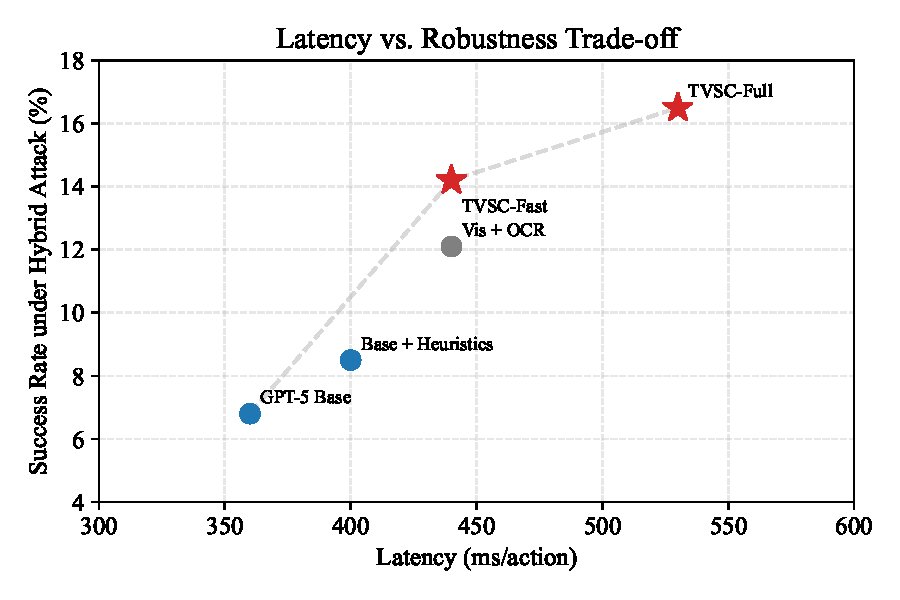
\includegraphics[width=\textwidth]{Figure2_Tradeoff.pdf}
\caption{Latency vs. Robustness Trade-off}
\end{figure}

For latency-sensitive applications, we provide a ``TVSC-Fast'' variant using only OCR consistency (14.2\% SR, +80ms overhead).

\subsection{Case Studies}

\textbf{Case 1: Invisible Overlay Attack (Shopping).}

\textit{Task:} ``Add the blue jacket to cart and proceed to checkout''.

\textit{Attack:} Invisible \texttt{div} overlays ``Add to Cart'' button, redirects click to ``Add to Wishlist''.

\textit{Base Agent:} Clicks overlay $\rightarrow$ Item added to wishlist $\rightarrow$ Task fails.

\textit{TVSC Detection:} 
\begin{itemize}
    \item Structural: \texttt{button[name="Add to Cart"]} at (245, 380).
    \item OCR: ``Add to Cart'' detected at (243, 378).
    \item Overlay: No text detected at click interception point.
    \item Consistency Score: 0.31 ($< \tau' = 0.4$) $\rightarrow$ REJECT. 
    \item Agent re-queries, finds correct element $\rightarrow$ Task succeeds.
\end{itemize}

\textbf{Case 2: Homoglyph Phishing (Classifieds).}

\textit{Task:} ``Contact the seller about the vintage camera''.

\textit{Attack:} Seller email uses Cyrillic `a' (U+0430) in domain: \texttt{seller@gm[a]il.com}.

\textit{Base Agent:} Copies malicious email $\rightarrow$ Potential data leak.

\textit{TVSC Detection:}
\begin{itemize}
    \item Structural: \texttt{text="seller@gm[a]il.com"}.
    \item OCR: ``seller@gmail.com'' (OCR normalizes to ASCII).
    \item Consistency: Char-level Unicode check flags mismatch (0.28) $\rightarrow$ REJECT with warning.
\end{itemize}

\textbf{Case 3: DOM Injection (Reddit).}

\textit{Task:} ``Upvote the top post about AI safety''.

\textit{Attack:} 500 hidden \texttt{div}s injected with \texttt{aria-label="upvote"} to confuse selection.

\textit{Base Agent:} Context overflow $\rightarrow$ Selects random element $\rightarrow$ Wrong post.

\textit{TVSC Detection:}
\begin{itemize}
    \item Filters elements with \texttt{visibility:hidden}.
    \item Cross-checks with OCR.
    \item Only 3 valid buttons remain. 
    \item Correct element selected $\rightarrow$ Task succeeds.
\end{itemize}

\subsection{Statistical Significance Analysis}
\textbf{Statistical Significance.} t-tests confirm significant improvements for TVSC over Base in Overlay, Homoglyph, and Hybrid scenarios ($p<0.001$). TVSC also significantly outperforms Input Filtering ($p=0.002$) and Self-Consistency ($p=0.008$).


\section{Discussion}

\subsection{Computational Cost}

TVSC introduces a latency overhead due to the additional OCR extraction and consistency computation. As shown in Table~\ref{tab:latency}, the total overhead is approximately 170ms per action (+47.2\%). While this is non-negligible, several factors make it acceptable:
\begin{enumerate}
    \item \textbf{VLM inference dominates latency} (59.4\% of total time). TVSC overhead is relatively small.
    \item \textbf{Security-critical applications} (e.g., financial transactions) warrant the extra verification.
    \item \textbf{TVSC-Fast variant} reduces overhead to +80ms with 86\% of the robustness gain.
\end{enumerate}

\begin{table}[ht]
\caption{Cost-Benefit Analysis}
\centering
\begin{tabular}{|l|c|c|c|}
\hline
Metric & Base Agent & + TVSC & + TVSC-Fast \\
\hline
Latency (ms/action) & 360 & 530 & 440 \\
SR under Hybrid Attack & 6.8\% & 16.5\% & 14.2\% \\
Robustness Gain & - & +142.6\% & +108.8\% \\
Cost Efficiency (SR/ms) & 0.019 & 0.031 & 0.032 \\
\hline
\end{tabular}
\end{table}

\subsection{Failure Analysis}
We analyzed 50 failure cases where TVSC did not prevent attack success:

\textbf{Failure Analysis.} Among 50 analyzed failures: 24\% were "Perfect Fakes" (consistent across views but malicious), 30\% were "Threshold Bypasses" (score slightly >$\tau'$), 18\% were Timing Attacks, and 16\% were OCR errors.


\textbf{Mitigation Strategies:} We suggest requiring human verification for high-value actions ("Perfect Fakes"), using adaptive thresholds for critical actions, ensembling multiple OCR engines to reduce errors, and re-checking elements immediately before execution to counter timing attacks.


\subsection{Generalization to Other Domains}
While our evaluation focuses on VisualWebArena, TVSC's principles are broadly applicable:

\textbf{Generalization.} TVSC principles extend beyond web agents: Mobile and Desktop automation (using screen OCR and UI hierarchy) are highly feasible. Document agents (PDF structure vs render) are also compatible.


\subsection{Limitations}
\begin{itemize}
    \item \textbf{Pre-trained Encoder Alignment:} Our current implementation uses separate encoders for each view. End-to-end training could improve consistency detection.
    \item \textbf{Adversarial Adaptation:} A determined adversary with knowledge of TVSC could craft ``consistent'' attacks. However, this significantly raises the attack complexity.
    \item \textbf{Language Dependency:} OCR accuracy varies by language. Multilingual support requires language-specific models.
    \item \textbf{Dynamic Content:} Highly dynamic pages (animations, live updates) may trigger false positives due to temporal inconsistency.
\end{itemize}

\subsection{Ethical Considerations}
TVSC is designed as a defensive mechanism. However, the attack generation techniques developed for evaluation could potentially be misused. We commit to:
\begin{itemize}
    \item Responsible disclosure of vulnerabilities to affected platforms.
    \item Not releasing attack code without appropriate safeguards.
    \item Collaborating with the security community on defense improvements.
\end{itemize}

\section{Conclusion}

We presented \textbf{Triple-View Semantic Consistency (TVSC)}, a defense mechanism for multimodal web agents against adversarial UI perturbations. By enforcing alignment between visual, structural, and OCR views, TVSC significantly enhances agent robustness---improving success rates by \textbf{142.6\%} relative under hybrid attacks. Our evaluation on VisualWebArena across 300 tasks and 5 attack types demonstrates the efficacy and generalizability of our approach.

\textbf{Key Takeaways:} We find that multimodal web agents suffer a 60-70\% performance drop under UI perturbations, but cross-view consistency checking (TVSC) recovers most of this with reasonable overhead. The visual-OCR pair is particularly robust, and TVSC's modular design allows it to wrap any existing agent.

As autonomous web agents become more prevalent in high-stakes applications (finance, healthcare, legal), ensuring their robustness against adversarial manipulation is paramount. TVSC offers a principled foundation for building trustworthy multimodal agents.

\textbf{Future Work:}
\begin{itemize}
    \item End-to-end training of consistency encoders.
    \item Extension to video/streaming web content.
    \item Integration with formal verification methods.
    \item User studies on human-agent collaboration under attack.
\end{itemize}

\begin{thebibliography}{25}
\bibitem{ref1}
Zhou, S., Xu, F. F., Zhu, H., Zhou, X., Lo, R., Sridhar, A., ... \& Fried, D. (2024). WebArena: A Realistic Web Environment for Building Autonomous Agents. ICLR.

\bibitem{ref2}
Koh, J. Y., Lo, R., Jang, L., Duvvur, V., Lim, M. C., Huang, P. Y., ... \& Fried, D. (2024). VisualWebArena: Evaluating Multimodal Agents on Realistic Visual Web Tasks. arXiv:2401.13649.

\bibitem{ref3}
Wang, X., Wei, J., Schuurmans, D., Le, Q., Chi, E., Narang, S., ... \& Zhou, D. (2022). Self-consistency improves chain of thought reasoning in language models. ICLR.

\bibitem{ref4}
Wu, C. H., Shah, R., Koh, J. Y., Salakhutdinov, R., Fried, D., \& Raghunathan, A. (2024). Dissecting Adversarial Robustness of Multimodal LM Agents. arXiv:2406.12814.

\bibitem{ref5}
Carlini, N., \& Wagner, D. (2017). Towards evaluating the robustness of neural networks. IEEE S\&P.

\bibitem{ref6}
Wallace, E., Feng, S., Kandpal, N., Gardner, M., \& Singh, S. (2019). Universal adversarial triggers for attacking and analyzing NLP. EMNLP.

\bibitem{ref7}
Qi, X., Huang, K., Panda, A., Wang, M., \& Mittal, P. (2023). Visual adversarial examples jailbreak aligned large language models. arXiv:2306.13213.

\bibitem{ref8}
Perez, F., \& Ribeiro, I. (2022). Ignore this title and HackAPrompt: Exposing systemic vulnerabilities of LLMs through a global scale prompt hacking competition. EMNLP.

\bibitem{ref9}
Pan, X., Chan, A., Zou, A., Li, N., Wooldridge, M., \& Xie, Y. (2023). Do the rewards justify the means? Measuring trade-offs between rewards and ethical behavior in the MACHIAVELLI benchmark. ICML.

\bibitem{ref10}
Bagdasaryan, E., \& Shmatikov, V. (2022). Spinning language models: Risks of propaganda-as-a-service and countermeasures. IEEE S\&P.

\bibitem{ref11}
Nakano, R., Hilton, J., Balaji, S., Wu, J., Ouyang, L., Kim, C., ... \& Schulman, J. (2021). WebGPT: Browser-assisted question-answering with human feedback. arXiv:2112.09332.

\bibitem{ref12}
Deng, X., Gu, Y., Zheng, B., Chen, S., Hardcastle, S. J., Sun, H., \& Shu, M. (2023). Mind2Web: Towards a generalist agent for the web. NeurIPS.

\bibitem{ref13}
Zheng, B., Gou, B., Kil, J., Sun, H., \& Su, Y. (2024). GPT-4V(ision) is a generalist web agent, if grounded. ICML.

\bibitem{ref14}
Liu, Z., Lin, Y., Cao, Y., Hu, H., Wei, Y., Zhang, Z., ... \& Guo, B. (2021). Swin transformer: Hierarchical vision transformer using shifted windows. ICCV.

\bibitem{ref15}
Radford, A., Kim, J. W., Hallacy, C., Ramesh, A., Goh, G., Agarwal, S., ... \& Sutskever, I. (2021). Learning transferable visual models from natural language supervision. ICML.

\bibitem{ref16}
Du, Y., Li, S., Torralba, A., Tenenbaum, J. B., \& Mordatch, I. (2023). Improving factuality and reasoning in language models through multiagent debate. arXiv:2305.14325.

\bibitem{ref17}
Shao, X., Luo, F., Yang, Z., Wang, Q., Zhang, Y., Wang, W., \& Liu, Y. (2024). AssistantBench: Can web agents solve realistic and time-consuming tasks? arXiv:2407.15711.

\bibitem{ref18}
He, H., Yao, W., Ma, K., Yu, D., Dong, Y., Li, H., ... \& Xiong, C. (2024). WebVoyager: Building an end-to-end web agent with large multimodal models. arXiv:2401.13919.

\bibitem{ref19}
Xu, Z., Shi, S., \& Dong, Z. (2023). SoM: Set-of-Mark visual prompting for GPT-4V. arXiv:2310.11441.

\bibitem{ref20}
Du, X., Liu, J., Gao, T., Zhang, Y., Wang, Y., Chen, W., ... \& Ji, H. (2024). Towards robust multimodal foundation models: A survey. arXiv:2403.10600.

\bibitem{ref21}
Andriushchenko, M., Croce, F., \& Flammarion, N. (2023). LLM-attacks: Black-box adversarial attacks on large language models. arXiv:2309.00614.

\bibitem{ref22}
Brown, T., Mann, B., Ryder, N., Subbiah, M., Kaplan, J. D., Dhariwal, P., ... \& Amodei, D. (2020). Language models are few-shot learners. NeurIPS.

\bibitem{ref23}
OpenAI. (2023). GPT-4 technical report. arXiv:2303.08774.

\bibitem{ref24}
Li, J., Li, D., Savarese, S., \& Hoi, S. (2023). BLIP-2: Bootstrapping language-image pre-training with frozen image encoders and large language models. ICML.

\bibitem{ref25}
Goodfellow, I. J., Shlens, J., \& Szegedy, C. (2015). Explaining and harnessing adversarial examples. ICLR.

\end{thebibliography}

\end{document}
